\documentclass{article}

\usepackage{hyperref}
\usepackage{graphicx}
\usepackage{natbib}

\begin{document}

\section{Alkoholkonsum in Baden Württemberg}



\subsection{Im zeitlichen Verlauf}
Schon im alten Griechenland wird in vielen Erzählungen über Saufgelage berichtet (TODO Quelle), damals war der Alkohol im Alltag allerdings verpönt (TODO Quelle). Erst seit dem Mittelarlter spielt Alkohol eine große Rolle in Europa. Ab dem ?? Jahrhundert wird er als ein wichtiger Teil der Ernährung von allen Altersgruppen mit etwa 3 Litern täglich Konsumiert (TODO Quelle). Man muss aber beachten, dass die Art dies Alkohols, die damals konsumiert wurde stark von heute abweicht. Ein großer Teil des Alkohols wurde z.B. in Form von Biersuppen konsumiert (TODO Quelle), bei deren Kochvorgang allerdings der Alkoholgehalt stark sank (TODO Quelle). Zu Beginn des 17. Jahrhunderts verbreiteten sich neue Genussmittel wie Kaffee, Kakao und Zucker in Europa, was zu einem starken Abfall des Alkoholkonsums führte (TODO Quelle). 

\subsection{Im vergleich zu anderen Bundesländern}
Viele haben das Vorurteil, dass zwischen dem Trinkverhalten in den nördlichen und den südlichen Bundesländern in Deutschland ein großes Gefälle besteht. Ein Beispiel dafür ist zum Beispiel das bayrische Oktoberfest, bei dem enorme Mengen an Alkohol konsumiert werden. Es wird auch als das größte Drogenfestival in Deutschland bezeichnet (TODO Quelle). Die Wissenschaft ist sich allerdings uneinig ob dieses Vorurteil wirdklich zutrifft. Es gibt Studien die behaupten, dass es durchaus ein Gefälle zwischen dem Trinkverhalten im Norden und im Süden Deutschlands gibt (TODO Quelle @Regionale Unterschiede in der Prävalenz riskanten Alkoholkonsums: Sekundäranalyse des Gesundheitssurveys Ost-West). Eine andere Studie behauptet wiederum, dass diese Differenzen nur durch falsche Datenerhebung hervorgerufen werden (TODO Quelle Der Einfluss regionaler Unterschiede im Trinkstil auf riskanten Konsum, exzessives Trinken, Missbrauch und Abhängigkeit). Um diese Behauptungen genauer zu analysieren haben wir die Methoden dieser Studien untersucht: 
\subsubsection {....}
Dafür müssen wir zuerst definieren, welche Bundesländer zu Nord- und Süd- Deutschland gehörren.... 
Metrik mit der gemessen wird: Menge an konsumiertem Reinalkohol (pro Trinktag ??)
....
Ergebniss: Es gibt keine Messbare differenz in der Menge an konsumierten reinalkohol zwischen Nord und Süddeutschland
---

Wenn man allerdings die einzelnen Bundesländer genauer betrachtet fällt auf, dass in Bayern tatsächlich überdurchschnittlich viel Alkohol konsumiert wird (TODO zitate und tabelle aus: @Der Einfluss regionaler Unterschiede im Trinkstil auf riskanten Konsum, exzessives Trinken, Missbrauch und Abhängigkeit). In Baden Württemberg wird allerdings durchschnittlich relativ wenig Alkohol pro Tag getrunken. Auch der riskante Alkoholkonsum ist relativ gering. (Verlgeich mit eigener Krankenhausstatistitk). Da wir uns in unserer Seminararbeit hautpsächlich auf den Alkoholkonsum von Jugendlichen fokussieren wollen wäre eine Statistik zum durchschnittlichen Alkoholkonsum von Jugendlichen in den verschiedenen Bundesländern natürlich interessant (TOOD vlt positiver formulieren). Bei unserer Rechere haben wir eine solche spezifische statistik allerdings nicht gefunden. 

Um aber trotzdem eine Aussage über den Alkoholkonsum von Jugendlichen in Deutschland zu treffen, haben wir die Daten auf der Plattform GENESIS (Gemeinsames Neues Statistisches Informations-System) (https://www-genesis.destatis.de/genesis/online) verwendet. Auf GENESIS findet sich ein breit  gefächertes Datenangebot von dne statistischen Landesämtern und dem Statistischen Bundesamt. Dieses enthält u.a. einen Datensatz mit dem Bundesland, Alter, Geschlecht und der Hauptdiagnose aller Krankenhauspatienten in Deutschland (\url{https://www-genesis.destatis.de/genesis//online?operation=table&code=23131-0011&bypass=true&levelindex=0&levelid=1707846572401#abreadcrumb}). Aus dieser Statistik haben wir alle Krankenhausaufenthalte von Jugendlichen bis 19 Jahren, die aufgrund von einer Alkoholintoxikation (Diagnose ICD-10 F10.0 (https://gesund.bund.de/icd-code-suche/f10-0)) im Krankenhaus waren extrahiert. In der folgenden Grafik sieht man diese im Durchschnitt pro 100.000 Einwohner des jeweiligen Bundeslandes über die letzten 15 Jahre aufgelistet.

\begin{figure}[h]
    \centering
    \includegraphics[scale=.7]{"assets/Alkohol_Bundesländer_avg_15_Jahre.png"}
    \caption{Alkoholbedingte Krankenhausaufenthalte von Jugendlichen in Abhängigkeit des Bundeslandes}
    \label{fig}
\end{figure}

Für die Bevölkerungsanzahlen zur normalisierung der Statistik wurde die Bevölkerung des jeweiligen Bundeslandes zum jeweiligen Zeitpunkt verwendet. (\url{https://www-genesis.destatis.de/genesis//online?operation=table&code=12411-0011&bypass=true&levelindex=0&levelid=1711822317197#abreadcrumb}). Die Werte wurden mit Python berechnet und die Grafik wurde mit der Python Bibliothek Matplotlib (https://matplotlib.org/) erstellt. 

Es fällt auf, dass die Werte für kleine Bundesländer (Saarland, Hamburg und Berlin) stark abweichen. Das könnte an den geringen Fallzahlen liegen, die dann zu Extremwerten führen. Die absoluten Fallzahlen schwanken im zum Beispiel Saarland über die Jahre von 200 bis knapp 400. Ein weiterer wichtiger Aspekt, der bei der Analyse dieser Daten beachtet werden muss, ist der Länderaustausch von Patienten. Das Bundesland, in dem ein Patient behandelt werden muss, muss nicht mit dem Wohnort des Patienten übereinstimmen. Das kann aufgrund der normalisierung der Daten zu einer verfälschung der Ergebnisse führen. Auf GENESIS ist auch eine Statistik verfügbar, die statt dem Ort des Krankenhauses den Wohnort der Patienten angibt (TODO Quelle \url{https://www-genesis.destatis.de/genesis//online?operation=table&code=23131-0003&bypass=true&levelindex=0&levelid=1711819504204#abreadcrumb}).

\begin{figure}[h]
    \centering
    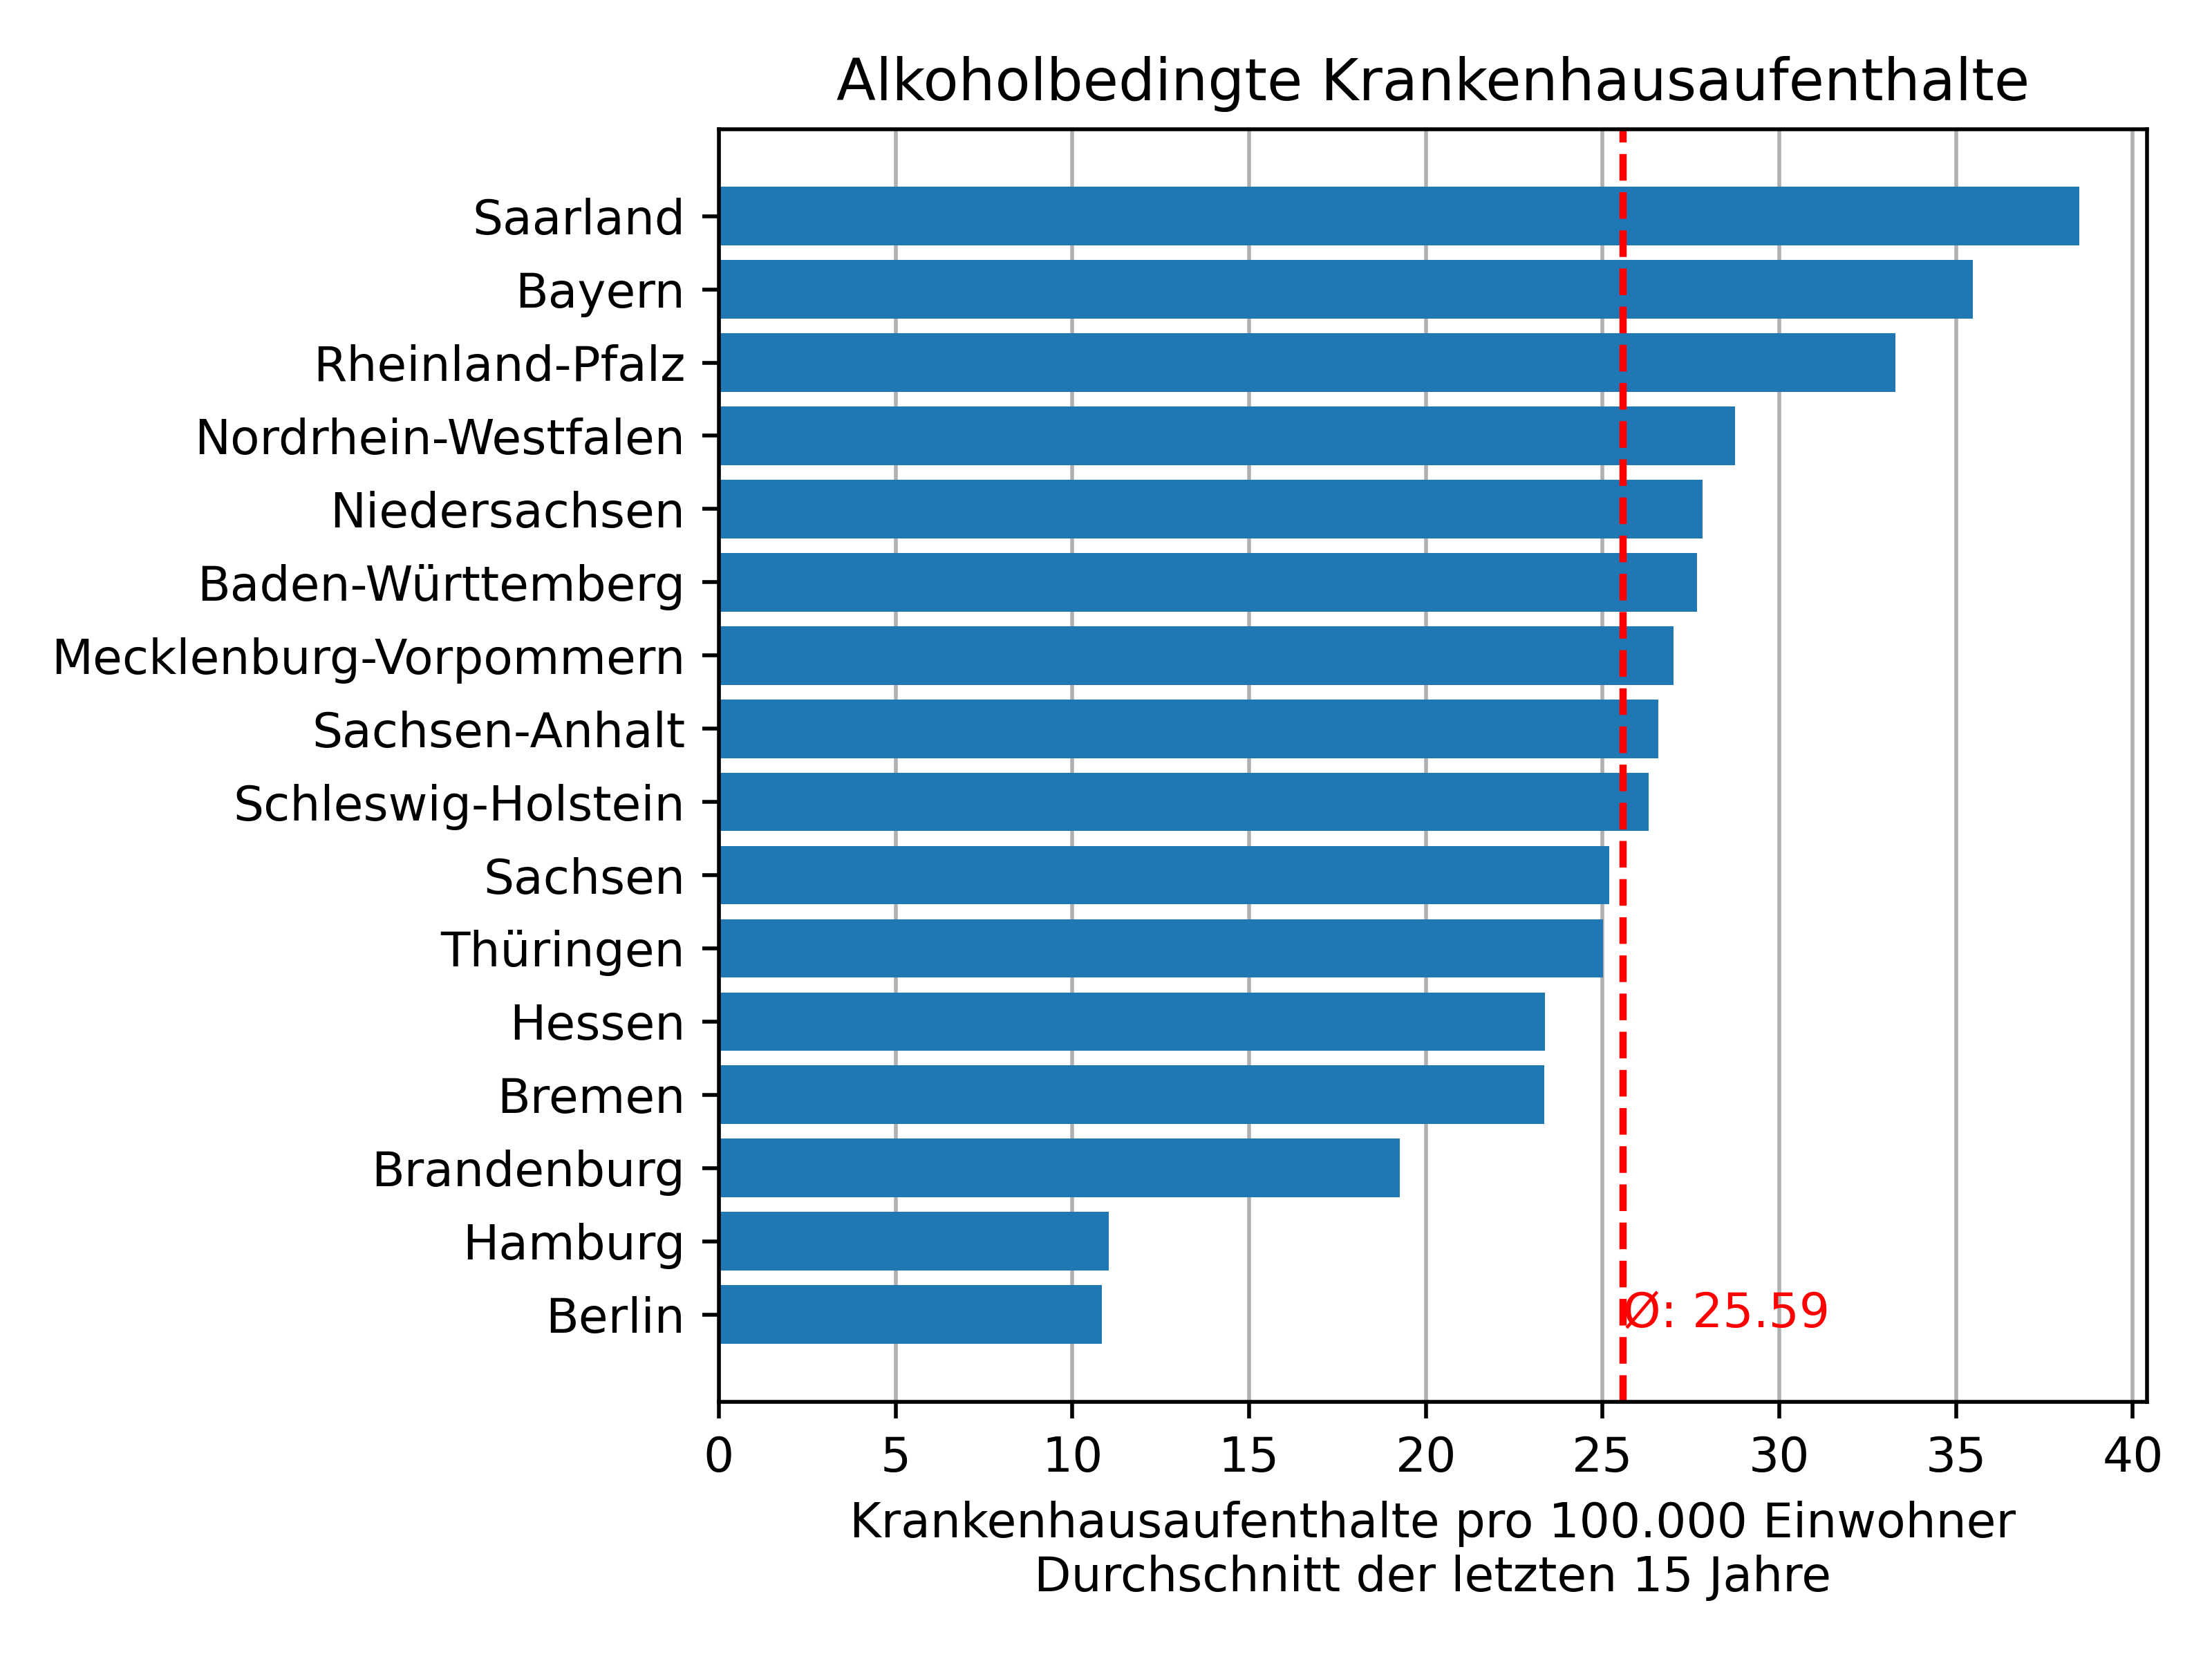
\includegraphics[scale=.7]{"assets/Alkohol_Wohnort_avg_15_Jahre.png"}
    \caption{Alkoholbedingte Krankenhausaufenthalte von Jugendlichen in Abhängigkeit des Wohnortes}
    \label{fig}
\end{figure}

\ref{fig:2} wurde mit den gleichen Methoden wie \ref{fig:1} erstellt. Patienten deren Wohnort unbekannt ist und Patienten, die aus dem Ausland kommen wurden ignoriert. 

Die Werte für die meisten größeren Bundesländer sind nahezu gleich geblieben, da dort der Anteil der Patienten, die in einem anderen Bundesland behandelt wurden im vergleich zu den Patienten, die in ihrem Heimatbundesland behandelt wurden sehr klein ist. Die Werte der kleineren Bundesländer (Hamburg, Berlin, Bremen und Saarland) sind dagegen stärker gesunken, vor allem bei Bremen. Das könnte daran liegen, dass ein Teil der Patienten, die zum Beispiel in einem Krankenhaus in Bremen behandelt wurden aus dem umliegenden Niedersachsen kommen. Dass die hohen Werte im Saarland kein Fehler in der Statistik sind, sondern ein reales Problem darstellen zeigt sich auch in diesem Artikel (TODO Quelle TODO vlt besserer Artikel https://jugendhilfeportal.de/artikel/saarland-zahl-der-wegen-alkoholmissbrauchs-akut-im-krankenhaus-behandelten-jugendlichen-weiter-gestiegen), der das Problem des alkoholmissbrauchs von Jugendlichen im Saarland beschreibt. 



\end{document}
